\section{Model Description}
\label{sec:KPCNet}

\begin{figure}[htbp]
  \centering
  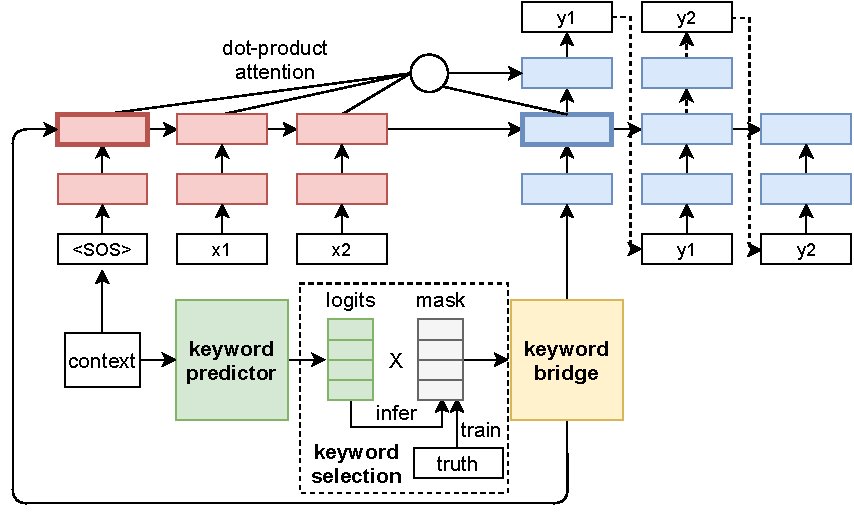
\includegraphics[width=1\linewidth]{kwd_model.pdf}
  \caption{Illustration of KPCNet.}
  \label{fig:pipeline}
  \end{figure}

  In Equation \ref{equ:decompose}, $p(\mathbf{z}|\mathbf{x})$ corresponds to the keyword prediction part, and $p(\mathbf{y}|\mathbf{x},\mathbf{z})$ refers to the keyword conditioned generation. Our model is thus divided into 2 logical parts. The whole model pipeline is illustrated in Figure \ref{fig:pipeline}.  

\subsection{Keyword Prediction}
\label{sec:prediction}

For the \textit{Keyword Predictor}, we assume the probability of each keyword $z$ are independent from each other given context $\mathbf{x}$, i.e. $p(\mathbf{z}|\mathbf{x})=\Pi_{z \in \mathbf{z}}p(z|\mathbf{x})$, to simplify the modeling. We parameterize $p(z|\mathbf{x})$ with TextCNN \citep{kim-2014-convolutional}. The training loss is binary cross entropy over each keyword: 


\begin{equation}
  L_{pred} = -\frac{1}{N}\sum_{n=1}^{N}\sum_{c=1}^{C}z^t_{n,c}log(p_{n,c})
  \label{equ:pred}
\end{equation}
Here we use $z^t_{n,c}$ as a binary indicator that shows if $c_{th}$ keyword in keyword dictionary $Z$ is among the ground truth keywords of the $n_{th}$ sample, and $p_{n,c}$ is the predicted probability for it.

\subsection{Keyword Conditioned Generation}
\label{sec:cond_gen}

The main structure of our generator is based on a standard sequence-to-sequence model \citep{luong2015effective}. We will focus on our specific design to condition the generation on keywords. 

\paragraph{Keyword Selection} We take the unnormalized keyword logits $\hat{p} \in \mathbb{R}^C$ from the keyword predictor, and then we select a conditioning keyword set $\mathbf{z}^s$ to mask out irrelevant dimensions to get a masked logits $\tilde{p} = [\hat{p}_1 z^s_1, \hat{p}_2 z^s_2, ..., \hat{p}_C z^s_C]$. This procedure allows us to control the generation with the selected keywords. Specific methods for this part will be discussed in \S \ref{sec:selection}.

\paragraph{Keyword Bridge} After getting the masked logits $\tilde{p}$, we pass them through a dropout layer, and then transform them to another distributed representation using a Multi-Layer Perceptron (MLP). They are then transformed into encoder features and decoder features with 2 MLPs respectively. The encoder feature will replace the hidden state of the first encoder step as memory to guide the generation via attention. The decoder feature will be fed as the input word embedding of the first decoder step to influence the generation.

\subsection{Keyword Selection}
\label{sec:selection}

At training, the ground truth keywords set $\mathbf{z}^t$ is selected as $\mathbf{z}^s$, and the training objective is to maximize the log-likelihood of all questions given context $\mathbf{x}$ and keywords $\mathbf{z}^t$. This equals to minimize: 

\begin{equation}
  L_{mle} = -\frac{1}{N}\sum^N_{n=1}log(p(\mathbf{y}_n|\mathbf{x}_n,\mathbf{z}^t_n))
  \label{equ:mle}
\end{equation}

At inference, we select $\mathbf{z}^s$ from keyword predictor's predicted distribution as condition for generation. This process was done once at a time, and can be done several times to fully explore the diversity in $p(\mathbf{y}|\mathbf{x})$ (Equation \ref{equ:decompose}) with different keyword sets. We come up with 3 methods for keyword selection:

\paragraph{Threshold} We select all keywords whose predicted probability are above a threshold $\alpha$ as $\mathbf{z}^s$. If not specified, this is the default selection method at inference.

\paragraph{Sampling} The threshold selection approach is deterministic and thus limited to one conditioning keyword set. We may encourage more diverse generation via diversifying the keyword set. An intuitive solution is to introduce randomness. Inspired by the Top-K \citep{fan-etal-2018-hierarchical, radford2019language} and Top-p (nucleus) sampling \citep{holtzman2019curious}, we also adopted a similar approach, sampling $k$ keywords from softmax-normalized prediction distribution after Top-K, Top-p filtering.

\paragraph{Clustering} Both the threshold and sampling selection strategies 
run the risk of putting semantically uncoherent keywords together, 
which is the drawback of the independence assumption used by keyword predictor. 
For example, if \textit{``voltage, machine, long, waffle''} are selected as 
the keywords for the waffle maker in Figure \ref{fig:WA_UI}, 
we may generate an illogical question ``what are the \textit{voltage} of 
the \textit{waffle}''. To get more coherent keyword sets, 
we explore the use of clustering technique. For the above example, 
the keywords can form 2 semantic groups, which lead to 
``What is the \textit{voltage} of the \textit{machine}'' and 
``How \textit{long} does it take to cook \textit{waffle}'', respectively. 

In practice, we first mine a keyword co-occurrence graph from the training set. We then take the Top-K likely keywords, and run Spectral clustering \citep{Shi00normalizedcuts} on the induced subgraph of them. The resulting $g$ disjoint groups are then used as generation conditions respectively.

\subsection{Keyword Controllability Probing}
\label{sec:probing}

One potential benefit that KPCNet brings is the controllability over 
generation by providing different conditioning keywords. To probe into this, 
we propose 2 approaches to operate on the keywords besides the 3 keywords 
selection methods. The operations are designed with hypotheses that 
will be tested with experiments.

\begin{table}[th]
  \small
  \centering
\begin{tabular}{l|l}
\hline
Product & \makecell[l]{iliving organic buckwheat pillow with authentic \\ japanese pillow cover, 14 by 20-inch, green } \\
\hline
KPCNet & \makecell[l]{what is the \textbf{size} of this \textbf{pillow} case? \\ (size, cover, pillow, wash, zipper)} \\
+Filter        & \makecell[l]{does this \textbf{pillow} have a \textbf{zipper}? \\ (cover, pillow, wash, zipper)} \\
\hline
\end{tabular}
\caption{\label{tab:kwd-filter} Example on the effect of keyword filtering. Predicted keywords for a question are shown in the parentheses below. ``size'' was filtered as it has already been covered in product description.}
\end{table}

\subsubsection{Keyword Filtering} \label{para:filter} Asking only about
things \textbf{not} in the context is the basic requirement of CQGen. 
However, none of existing methods in the literature 
have specific solution for this. In preliminary experiments of KPCNet, 
we found that some of the repetitive cases came with repetitive keywords.
Therefore, we conjecture that we may alleviate the problem by filtering 
out such repetitive keywords. Table \ref{tab:kwd-filter} provided a 
concrete example. This would be especially useful for iterative generation, 
as we will explicitly exclude repeating keywords if user triggers CQGen 
for the second time with some information vacancy already filled.

Here we use a simple matching method for keyword filtering. 
We first select a set of keywords that tends to lead to repetition. 
Then for each keyword in the set, we maintain a blacklist of words or 
patterns so that we filter the keyword if the pattern is matched. 
For example, we would filter words like ``height''/``width'' from the predicted keywords, if we can match ``height''/``width'' in the context. 
This process is currently done manually, so it doesn't scale. 
However, we find that a small set of frequent keywords is already 
enough to cover a relatively large number of repetitive cases and 
demonstrate the effect of this approach, as will be shown in \S \ref{sec:experiments}. 
We leave automatic repeating keyword detection and filtering for future works.  


\subsubsection{External Knowledge} \label{sec:knowledge}
It is a common practice for e-commerce platforms to build knowledge graph 
to manage their products~\citep{dong2018challenges, luo2020alicoco}. 
As a result, products are attached to highly related tags, concepts, 
or keywords in our terms. Since the keywords used here is just a simple kind of knowledge, we believe that such richer external knowledge may further improve the generation by directly providing high-quality keywords, or helping the keyword prediction. Nevertheless, since we don't have access to such knowledge, we simulate such scenario where we have higher quality keywords by directly feeding ground truth keywords to the model[KPCNet(truth)]. This establishes an upper bound to what extent can KPCNet be improved with knowledge.

\subsection{Deduplication Postprocessing}
\label{sec:deduplicate}
All algorithms will more or less produce semantically similar questions 
in their initial generation group. Therefore, we will first generate 
more candidates than needed (say, produce 6 questions for 3 displaying slots), 
so that at least certain level of diversity can be guaranteed for 
the initial group. We then apply a simple, model-agnostic heuristic for 
deduplicating question selection. We first add the top generation into 
the current group, then we will iterative through the remaining questions. 
If the question's Jaccard similarity with any currently selected question 
is below 0.5, it will be added into the current group, otherwise 
it will be discarded. 

